\documentclass[conference]{IEEEtran}
\IEEEoverridecommandlockouts
\usepackage[T1]{fontenc}
\usepackage{cite}
\usepackage{amsmath,amssymb}
\usepackage{graphicx}
\usepackage{booktabs}
\usepackage{url}
\usepackage{xcolor}
\usepackage{tikz}
\usetikzlibrary{positioning,arrows.meta,fit}

\begin{document}
\bstctlcite{IEEEexample:BSTcontrol}

\title{Shielding Medical Loads: Hard-Constraint Energy Management for Elderly Households in Heatwave Power Outages}

\author{\IEEEauthorblockN{Author Name(s)}
\IEEEauthorblockA{\textit{Department} \\
\textit{Institution}\\
City, Country \\
email@institution.edu}}

\maketitle

\begin{abstract}
Older adults who rely on electrically powered medical equipment face acute risk when heatwaves and power outages coincide. Energy-management systems for such households usually encode medical priority as a weight in an objective or reward, which trades it against comfort and cost. We argue that medical service should instead be a hard constraint, and propose the CareGrid shield: a runtime safety layer that wraps any dispatch policy, serves critical devices first, and locks a battery reserve sized to carry them to a worst-case restoration time. We evaluate it on two independent simulation platforms driven by real data: a community microgrid of eight elderly households and a care facility under the July 2023 Phoenix heatwave (ERA5 weather, NREL ResStock loads; 6,048 outages), and ten ResStock homes in CityLearn v3 with LSTM thermal models and measured 2018 Austin weather (2,016 episodes). Across outages of 12--72\,h, with the controller told that restoration would take 24\,h, the shield reduced unpowered medical device-hours from 103.8 to 0 (Phoenix) and from 81.4 to 6.1 (CityLearn) relative to the same controller with weighted priority. The price was 6\% and 25\% more resident heat exposure, respectively. A model-predictive controller with weighted priority was nearly safe at its default weights but lost 386 device-hours per 48\,h outage when the weight on cooling was doubled; inside the shield it lost none at any weight tested.
\end{abstract}

\begin{IEEEkeywords}
Energy resilience, power outages, older adults, safe reinforcement learning, shielding, microgrids, demand response
\end{IEEEkeywords}

\section{Introduction}
Heatwaves and power outages increasingly arrive together, and the combination is far more dangerous than either alone. Across U.S. counties from 2015 to 2019, each hour of outage on a hot day increased the mortality harm of that day by 61\%, with the elderly among the groups most affected \cite{ai2025heat}. Modelling of historical heatwaves suggests that a multiday blackout during a heatwave would more than double heat-related mortality and would require medical attention for more than half of Phoenix's population \cite{stone2023blackouts}. Outages are also associated with cardiovascular and respiratory hospitalizations among Medicare beneficiaries \cite{mcbrien2026outages}. More than 4.5 million U.S. Medicare beneficiaries living independently rely on electricity-dependent medical equipment or services \cite{empower}, and rentals of such equipment more than doubled across most demographic groups between 2008 and 2018 \cite{casey2021dme}. Outage vulnerability is unevenly distributed \cite{dugan2025survey,ezzati2025porsvi}, and older people face distinct risks in the energy transition \cite{zuk2024ageism}.

Rooftop solar, home batteries and community microgrids can bridge outages, but they do not remove the allocation problem: when an islanded system runs short, something has to be switched off, and the restoration time is unknown. Energy-management systems designed for older adults optimise comfort and cost while the grid is up \cite{athanasiadis2022sems,tsaknakis2023nearly,kaculi2025human}. Resilience-oriented controllers, including multi-agent reinforcement learning (MARL), maximise generic critical-load service or minimise cost \cite{wu2026marl,qiu2023repair,esan2026lean}. Gong \textit{et al.}\ showed that adding the settlement cost of durable-medical-equipment (DME) users to an offline load-shedding optimisation cut DME exposure by 77.6\% \cite{gong2026dilemma}. Across this work, vulnerability enters as a weight or cost term.

A weight is the wrong instrument for a life-safety requirement. Its effect depends on tuning, it is traded continuously against comfort, and it does not account for the uncertain length of the outage, which determines whether energy spent now is energy missing later. Safe reinforcement learning offers an alternative: constrained policy optimisation \cite{achiam2017cpo,stooke2020pid} and runtime shields that override unsafe actions \cite{alshiekh2018shield}.

This paper makes three contributions.
\begin{enumerate}
\item We formulate outage dispatch for elderly households as a lexicographic problem in which medical service is a hard constraint under restoration-time uncertainty, and propose a policy-agnostic runtime shield with a worst-case battery reserve and a solar refill rule.
\item We evaluate the shield on two independent platforms driven by real weather and building data, our calibrated simulator and CityLearn v3, in 8,064 simulated outages, against the status quo, a rule-based controller, weighted greedy and model-predictive controllers, and performance bounds.
\item We quantify the price of the guarantee in heat exposure and the sensitivity of weighted controllers to their weights, and we identify and work around an islanding limitation in CityLearn 3.0.2. Code and data pipelines are released.\footnote{Repository URL to be added for the camera-ready version.}
\end{enumerate}

\section{Related Work}
\textit{Energy management for older adults.} Athanasiadis \textit{et al.}\ \cite{athanasiadis2022sems} and Tsaknakis \textit{et al.}\ \cite{tsaknakis2023nearly} control thermal, storage and appliance loads in elderly households, using disaggregation to monitor activity. Kaculi \textit{et al.}\ \cite{kaculi2025human} design demand response around the comfort of aging occupants. Digital twins of older adults are emerging \cite{lehmann2024twins,momand2025twins}, but they are not yet coupled to energy dispatch. These systems assume a grid connection and treat comfort as an objective.

\textit{Microgrid resilience and learning.} MARL has been used to keep microgrids running through typhoons \cite{wu2026marl}, to dispatch repair crews \cite{qiu2023repair} and to manage networked microgrids under uncertainty \cite{esan2026lean}. Cognitive and edge-coordinated digital twins approach optimal microgrid operation in practice \cite{sivaneasan2025cognitive,vanitha2025cet}. None of these treats a person's medical equipment as a constraint.

\textit{Equity in load shedding.} Gong \textit{et al.}\ \cite{gong2026dilemma} is the closest work. They optimise a single offline curtailment decision with a DME-aware cost. We address online, hour-by-hour control of islanded resources under an uncertain restoration time, and we enforce medical service as a constraint rather than a cost.

\section{Problem Formulation and the CareGrid Shield}
\subsection{Islanded system}
A set of buildings $\mathcal{H}$ is islanded from hour $t_0$ until an unknown restoration time $\tau$. Building $h$ has $n_h$ residents and medical devices $\mathcal{D}_h$, each drawing $p_d(t)$ on its schedule (continuous for oxygen concentrators, nightly for CPAP). In each hour the controller chooses device states $x_{d,t}\in\{0,1\}$, essential-circuit power $e_{h,t}$ and cooling power $u_{h,t}$, subject to
\begin{gather}
\textstyle\sum_{h}\big(\sum_{d\in\mathcal{D}_h} x_{d,t}\,p_d(t) + e_{h,t} + u_{h,t}\big) + c_t = P_t + d_t - s_t, \\
E_{t+1} = E_t + \eta c_t - d_t/\eta, \\
E_{\min}\le E_t\le E_{\max},\qquad 0\le c_t,d_t\le \bar P,
\end{gather}
where $P_t$ is solar output, $E_t$ is battery energy, $c_t,d_t$ are charge and discharge, and $s_t\ge 0$ is curtailment. Indoor temperature follows a grey-box model
\begin{equation}
T_{h,t+1} = T_{h,t} + \tfrac{1}{C_h}\!\left[\tfrac{T^{o}_t - T_{h,t}}{R_h} + a_h G_t + q_h - \mathrm{COP}(T^{o}_t)\,u_{h,t}\right]
\end{equation}
(in CityLearn, by the platform's per-home LSTM instead).

\subsection{Objectives under restoration uncertainty}
We define unserved critical energy $J_1=\sum_t\sum_d p_d(t)(1-x_{d,t})$, resident heat exposure $J_2=\sum_t\sum_h n_h\,[T_{h,t}-T_c]^+$ with $T_c=26.7^\circ$C, and unserved essential energy $J_3$. The intended preference is lexicographic: minimise $J_1$, then $J_2$, then $J_3$. The controller knows the utility's point estimate $\hat\tau$ of restoration and a conservative bound $\tau_{90}$, but not $\tau$. A weighted controller minimises $w_c J_1 + w_h J_2 + w_e J_3$. A constrained controller minimises $J_2$ and $J_3$ subject to $J_1=0$ whenever that is feasible.

\subsection{The CareGrid shield}
The shield sits between any policy and the plant (Fig.~\ref{fig:shield}). Every hour it:
\begin{enumerate}
\item serves critical devices first from the available supply $S_t = P_t + \min(\bar P, \eta(E_t - E_{\min}))$, smallest device first;
\item computes a reserve that carries all devices to the worst-case restoration time, net of a conservative persistence forecast of solar output,
\begin{equation}
R_t = \sum_{k=1}^{H_t}\Big[\textstyle\sum_{d} p_d(t+k) - \alpha P_{t+k-24}\Big]^+,
\end{equation}
where $H_t=\max(H_{\min},\,\tau_{90}-t)$, $\alpha=0.7$ and $H_{\min}=12$\,h;
\item when stored energy is below $R_t$, routes surplus solar to the battery before any non-critical use;
\item passes the policy's non-critical proposal through only within the budget left above the reserve, paced to $\hat\tau$:
\begin{equation}
B_t=\min\!\Big\{S_t-\kappa_t,\;\tilde P_t+\min\!\big(\bar P-b_t,\;\tfrac{[E^{a}_t-b_t-R_t]^+}{\max(1,\hat\tau-t)}\big)\Big\},
\end{equation}
where $\kappa_t$ is the critical power served, $b_t$ the part of it drawn from the battery, $E^{a}_t$ the deliverable stored energy and $\tilde P_t$ the solar left after critical loads and refilling.
\end{enumerate}
The shield does not rank residents against one another. It guarantees each device a service floor, and it leaves the allocation of comfort to the policy it wraps, which can be a rule, an optimiser or a learned agent.

\begin{figure}[t]
\centering
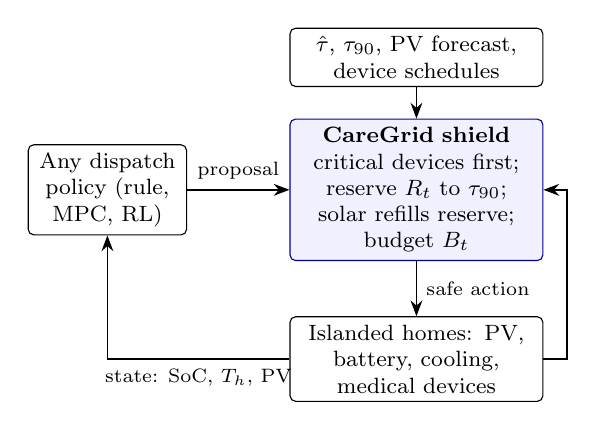
\begin{tikzpicture}[font=\footnotesize,
  box/.style={draw, rounded corners=2pt, align=center, inner sep=3pt, minimum height=8mm},
  arr/.style={-{Stealth[length=2mm]}, semithick}]
\node[box, text width=18mm] (pol) {Any dispatch\\policy (rule,\\MPC, RL)};
\node[box, right=13mm of pol, text width=30mm, fill=blue!6, draw=blue!60!black] (sh) {\textbf{CareGrid shield}\\critical devices first;\\reserve $R_t$ to $\tau_{90}$;\\solar refills reserve;\\budget $B_t$};
\node[box, above=4mm of sh, text width=30mm, minimum height=6mm] (fc) {$\hat\tau$, $\tau_{90}$, PV forecast,\\device schedules};
\node[box, below=7mm of sh, text width=30mm] (pl) {Islanded homes: PV,\\battery, cooling,\\medical devices};
\draw[arr] (pol) -- node[above, font=\scriptsize]{proposal} (sh);
\draw[arr] (fc) -- (sh);
\draw[arr] (sh) -- node[right, font=\scriptsize]{safe action} (pl);
\draw[arr] (pl.west) -| node[pos=0.25, below, font=\scriptsize]{state: SoC, $T_h$, PV} (pol.south);
\draw[arr] (pl.east) -- ++(3mm,0) |- (sh.east);
\end{tikzpicture}
\caption{The CareGrid shield wraps any dispatch policy. The policy proposes non-critical allocations; the shield enforces medical service and a worst-case reserve before passing them to the islanded system.}
\label{fig:shield}
\end{figure}

\section{Experimental Setup}
\subsection{Controllers}
\emph{Equal curtailment} (the status quo) scales all loads by the same fraction; a device receiving less than full power trips. \emph{Rule-based} serves critical devices, then essential circuits, and cools only while the battery is above 40\% or from instantaneous solar. \emph{Weighted greedy} ranks loads by value per kWh: $w_c=10$ for devices, 2 for essential circuits, and $w_h\rho_h$ for cooling, with $\rho_h = n_h[\tilde T_h - T_c]^+/(32.2^\circ\mathrm{C} - T_c)$, where $\tilde T_h$ is the indoor temperature expected without cooling (the current temperature in CityLearn); it paces the battery to $\hat\tau$. \emph{Weighted MPC} solves a receding-horizon linear program (HiGHS \cite{huangfu2018highs}) to $\hat\tau$ (at least 12\,h) with perfect weather and solar forecasts; we also test a critical weight of 1000 and a horizon of $\tau_{90}$. The \emph{shielded} variants wrap the greedy and MPC policies. As bounds we use a \emph{perfect-foresight} linear program that knows $\tau$ and relaxes device states to $[0,1]$, and, in CityLearn, \emph{medical-only} dispatch, which spends energy on nothing but medical devices.

\subsection{Platform 1: Phoenix community microgrid}
Eight households and a six-resident care facility (17 residents) share 12 medical devices: five 350\,W oxygen concentrators, a 150\,W ventilator, two 60\,W CPAP machines used at night, three 120--150\,W medication fridges and a 300\,W wheelchair charger. They share 60\,kWp of PV and a 150\,kWh, 60\,kW battery ($\eta=0.95$). Hourly temperature and irradiance for 30 June to 3 August 2023, peaking at 46.8$^\circ$C, come from ERA5 \cite{hersbach2020era5} via Open-Meteo \cite{zippenfenig2023openmeteo}. The non-cooling load shape is taken from NREL ResStock for Maricopa County \cite{wilson2022eulp}. The thermal model ($R_h=1.75^\circ$C/kW, $C_h=6$\,kWh/$^\circ$C per home-equivalent) uses 55.9\,kWh/day of cooling in July 2023, against 51.1\,kWh/day in ResStock for the cooler July 2018. Without cooling, indoor temperature reaches 39.5$^\circ$C within 8\,h on the hottest day. While grid-connected, the battery runs in self-consumption mode with a 30\% backup reserve.

\subsection{Platform 2: CityLearn v3}
We use CityLearn 3.0.2 \cite{fonseca2026citylearnv3,nweye2025citylearn} with its \texttt{tx\_travis\_county\_neighborhood} dataset: ResStock homes in Austin, TX, with per-home LSTM thermal models and measured 2018 weather. We take the first ten homes with summer cooling and give them the same kinds of households (14 residents, 12 devices). Each home has 6\,kW of PV, modelled with PVWatts v8 \cite{dobos2014pvwatts} on the dataset's weather file (1,388\,kWh/kW per year), and a 13.5\,kWh, 5\,kW battery. During outages each home runs a critical-loads panel (0.35\,kW of essential circuits plus its devices, water heater off), identical for every controller.

In CityLearn 3.0.2's built-in outage mode, batteries cannot discharge: discharge is capped by a local-load estimate that is computed before loads are energised and is net of solar, so it is zero. We therefore run CityLearn grid-connected and enforce islanding in the controller layer. During outage hours loads are served only from PV and battery, and any grid import that CityLearn still records is counted as unserved energy, charged to medical devices first. This mismatch averaged 0.25\,kWh per outage.

\subsection{Scenarios and metrics}
Outages begin at 14:00 local time on each of 1--28 July, with true durations of 12, 24, 48 and 72\,h. Every controller is told $\hat\tau=24$\,h, and the shield uses $\tau_{90}=48$\,h. Each scenario is run with and without a 24\,h warning, during which the battery is pre-charged. Sweeps vary the heat weight $w_h\in\{0.25,\dots,8\}$, battery size, $\tau_{90}$ and outage start hour. The primary metric is unpowered medical device-hours. We also report critical energy served, person-hours indoors above 32.2$^\circ$C (the National Weather Service ``extreme caution'' threshold) and person-degree-hours above 26.7$^\circ$C. Intervals are 95\% bootstrap intervals over start days, and comparisons use paired Wilcoxon signed-rank tests.

\begin{table*}[t]
\centering
\caption{Outage results without warning, pooled over 28 start days $\times$ 4 durations ($n=112$ per cell). Device-h: unpowered medical device-hours per outage. Crit.: critical energy served (\%). PH$_{32}$: person-hours indoors above 32.2$^\circ$C. PDH: person-degree-hours above 26.7$^\circ$C. --: not run on that platform.}
\label{tab:main}
\begin{tabular}{lrrrrrrr}
\toprule
 & \multicolumn{4}{c}{Phoenix community microgrid (Platform 1)} & \multicolumn{3}{c}{CityLearn v3, Austin (Platform 2)} \\
\cmidrule(lr){2-5}\cmidrule(lr){6-8}
Controller & Device-h & Crit.\ (\%) & PH$_{32}$ & PDH & Device-h & Crit.\ (\%) & PH$_{32}$ \\
\midrule
Equal curtailment (status quo) & 374.0 & 4.2 & 450 & 4{,}164 & 209.2 & 40.0 & 12 \\
Rule-based critical-first & 148.6 & 67.9 & 511 & 4{,}799 & 104.8 & 71.2 & 30 \\
Priority as weight, greedy & 103.8 & 82.0 & 409 & 4{,}073 & 81.4 & 81.4 & 32 \\
Priority as weight, MPC & 0.8 & 99.9 & 345 & 3{,}727 & -- & -- & -- \\
\quad MPC, critical weight $\times$100 & 0.8 & 99.9 & 345 & 3{,}727 & -- & -- & -- \\
\quad MPC planned to P90 & 0.3 & 100.0 & 336 & 3{,}723 & -- & -- & -- \\
\textbf{CareGrid shield, greedy} & 0.0 & 100.0 & 429 & 4{,}324 & 6.1 & 98.3 & 44 \\
\textbf{CareGrid shield + MPC} & 0.0 & 100.0 & 363 & 3{,}974 & -- & -- & -- \\
\textbf{CareGrid shield + P90 MPC} & 0.0 & 100.0 & 340 & 3{,}894 & -- & -- & -- \\
Medical-only dispatch (bound) & -- & -- & -- & -- & 2.2 & 99.0 & 340 \\
Perfect-foresight optimum (bound) & 0.0 & 100.0 & 320 & 3{,}613 & -- & -- & -- \\
\bottomrule
\end{tabular}
\end{table*}


\section{Results}
\subsection{Medical service}
Table~\ref{tab:main} summarises the results. With weighted priority, the greedy controller left medical devices unpowered for 103.8 device-hours per outage in Phoenix (95\% CI 85--122) and 81.4 in CityLearn (66.7--96.4). Inside the shield the same controller lost 0 and 6.1 (4.1--8.4) device-hours, respectively ($p=1.6\times10^{-15}$ and $p=8.5\times10^{-19}$). Equal curtailment, which treats all loads alike, lost 374 and 209 device-hours. Fig.~\ref{fig:duration} shows that the weighted controller degrades with outage length. Fig.~\ref{fig:case} shows why: on the hottest afternoon it spends the battery on cooling, runs dry overnight, and drops every medical device for hours, while the shield holds a reserve and indoor temperatures barely differ. In CityLearn the shield stays within 4 device-hours of the medical-only bound up to 48\,h; at 72\,h, beyond $\tau_{90}$, it loses 14.9 against the bound's 2.9.

\begin{figure}[t]
\centering
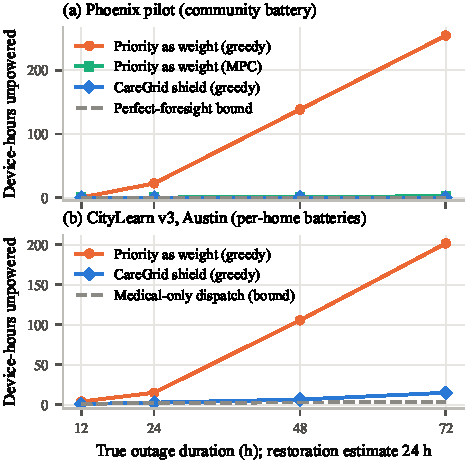
\includegraphics[width=\columnwidth]{fig_duration.pdf}
\caption{Unpowered medical device-hours against true outage duration (mean of 28 start days, no warning).}
\label{fig:duration}
\end{figure}

\subsection{Sensitivity of weighted priority}
A weighted MPC with perfect weather forecasts was nearly safe at its default weights (0.8 device-hours per outage), so forecasting and planning recover much of the gap. Its safety depended on the weights, however (Fig.~\ref{fig:tradeoff}). At 48\,h, doubling the heat weight raised its losses from 0.8 to 386 device-hours, and quadrupling it gave 472. Raising the critical weight a hundredfold did not remove the residual losses ($p=0.33$), and outages starting at 20:00 cost the unshielded MPC 39 device-hours. The shielded MPC planned to $\tau_{90}$ lost no device-hours at any weight, start hour or battery size tested. In CityLearn, which always serves base load before cooling within an hour, the weighted greedy controller lost 104--106 device-hours at every heat weight: its failures came from spending stored energy early, which no weight corrected.

\begin{figure}[t]
\centering
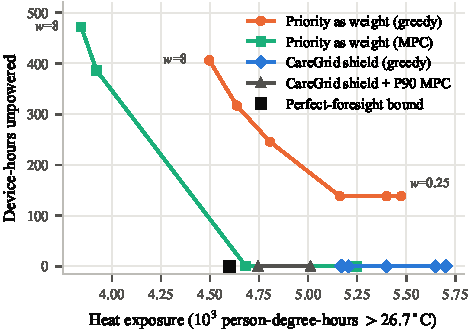
\includegraphics[width=\columnwidth]{fig_tradeoff.pdf}
\caption{Phoenix, 48\,h outages: heat weight $w_h$ swept from 0.25 to 8. Weighted controllers trade medical service for comfort; shielded controllers do not.}
\label{fig:tradeoff}
\end{figure}

\begin{figure*}[t]
\centering
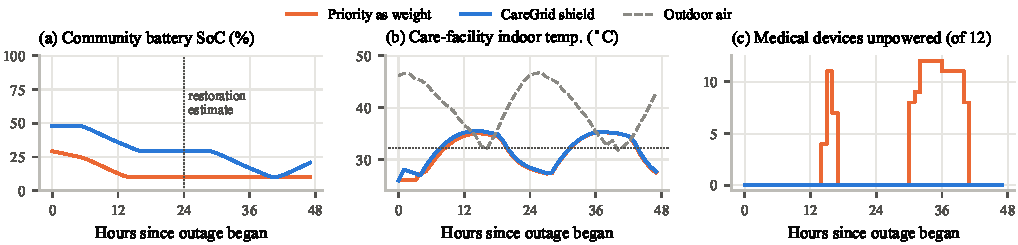
\includegraphics[width=\textwidth]{fig_case.pdf}
\caption{Phoenix case study: 48\,h outage from 14:00 on 19 July 2023, the hottest start of the month. The weighted controller exhausts the battery on the first evening and leaves up to all 12 medical devices unpowered; the shield keeps a reserve and every device powered, with almost the same indoor temperatures.}
\label{fig:case}
\end{figure*}

\subsection{Price of the guarantee and value of warning}
The reserve has a cost in comfort. In Phoenix, resident heat exposure rose by 6\% (4,073 to 4,324 person-degree-hours for greedy; 3,727 to 3,974 for MPC), and the best shielded controller came within 8\% of the perfect-foresight bound (3,894 against 3,613). In CityLearn, where each home holds its own 13.5\,kWh battery, the cost was larger: 25\% more person-degree-hours and 44 against 32 person-hours above 32.2$^\circ$C. Medical-only dispatch marks the extreme of this trade-off at 340 person-hours. A 24\,h warning, which raised the Phoenix battery from 30\% to full at a cost of 111\,kWh of grid energy, cut heat exposure by 11--19\% across controllers. In CityLearn it reduced shielded losses from 6.1 to 4.1 device-hours.

\section{Discussion and Limitations}
Weighted priority failed in three ways: through the within-hour ranking (when a hot home outranks an oxygen concentrator), through intertemporal spending under an uncertain restoration time, and through sensitivity to tuning that differed between platforms. A constraint enforced at run time removes all three without fixing the policy that sits inside it. The remaining gap to the bounds is a target for constrained, learned policies trained inside the shield \cite{achiam2017cpo,stooke2020pid}, and for a health twin that would direct cooling to the residents at greatest physiological risk \cite{momand2025twins}. Because the shield guarantees floors rather than ranking people, it is simpler to contest and to audit, which matters for a system that would likely be classed as high-risk AI in critical infrastructure.

These results come from simulation. The households are synthetic, each platform covers one city and one month at an hourly step, and neither includes distribution-network constraints. The Phoenix building model is calibrated on energy use, not on measured indoor temperatures. CityLearn's LSTMs were trained with working cooling. With cooling shed for long periods they predicted indoor peaks up to 47.3$^\circ$C, and 13\% of episodes peaked above 40$^\circ$C, mostly under medical-only dispatch. For that reason we emphasise hours above 32.2$^\circ$C, which is less sensitive to extreme values than degree-hours. The CityLearn result also relies on the islanding workaround described above.

\section{Conclusion}
Treating elderly residents' medical equipment as a hard, shielded constraint rather than a weighted objective eliminated or nearly eliminated medical-device outages across 8,064 simulated heatwave outages on two platforms driven by real data. It cost 6--25\% more heat exposure, a gap that better policies inside the shield can narrow. Next steps are constrained multi-agent RL within the shield, coupling a physiological health twin, and validation with metered data from homes and care facilities.

\bibliographystyle{IEEEtran}
\bibliography{refs}

\end{document}
